\documentclass[a4paper]{article}
\usepackage{amsmath}
\usepackage{amssymb}
\usepackage{graphicx}
\usepackage{verbatim}
\usepackage[bookmarks=true]{hyperref}
\usepackage[left=2cm, right=2cm]{geometry}
\usepackage{listings}
\usepackage[dvipsnames]{xcolor}

\definecolor{wow}{RGB}{73,63,72}
\usepackage{stix}
% \usepackage{newtxtext}
% \usepackage{eulervm}

\lstset{morecomment=[l]--,
  commentstyle=\color{NavyBlue},
        basicstyle=\small\ttfamily,
        numbers=left,
        classoffset=0,
        morekeywords={TODO},
        keywordstyle=\color{red}\bfseries,
        classoffset=1,
        morekeywords={class,
                      visible,
                      temporal,
                      TD,
                      TI, 
                      items,
                      modules,
                      connection,
                      predicates,
                      axioms,
                      end,
                      inherits,
                      vars},
        keywordstyle=\bfseries,
        classoffset=2,
        morekeywords={axioms},keywordstyle=\color{green},
        classoffset=0}%



\title{Politecnico di Milano\\
Formal Methods for Concurrent \\
and \\
Real-time Systems\\
Homework project\\
\textbf{Collaborative Robotics Modeling }}
\author{Aldeghi Gabriele \\
  Mantovani Mirko \and
  Sacco Alessio \\
  Sonzogni Stefano}
 \date{\today}
 



% The other logical operators are: \lnot, \land, \lor, \iff
\newcommand{\liff}{\iff}
\DeclareMathOperator{\limply}{\Rightarrow}
\DeclareMathOperator{\future}{Future}
\DeclareMathOperator{\past}{Past}
\DeclareMathOperator{\lastsOp}{Lasts}
\newcommand{\lasts}{\lastsOp_{ee}}
\newcommand{\lastsie}{\lastsOp_{ie}}
\newcommand{\lastsii}{\lastsOp_{ii}}
\newcommand{\lastsei}{\lastsOp_{ei}}
\DeclareMathOperator{\lastedOp}{Lasted}
\newcommand{\lasted}{\lastedOp_{ei}}
\DeclareMathOperator{\always}{Always}
\DeclareMathOperator{\sometimeFuture}{SometimeFut}
\DeclareMathOperator{\sometimePast}{SometimePast}
\DeclareMathOperator{\withinOp}{Within}
\newcommand{\within}{\withinOp_{ee}}
\DeclareMathOperator{\uptonow}{UpToNow}
\DeclareMathOperator{\becomes}{Becomes}
\DeclareMathOperator{\nexttime}{NextTime}
\DeclareMathOperator{\lasttime}{LastTime}
\DeclareMathOperator{\until}{Until}
\DeclareMathOperator{\since}{Since}


\begin{document}
\maketitle
\begin{center}
    
\includegraphics[width=7cm]{images/polimi-logo}
\end{center}
\clearpage
{\hypersetup{hidelinks}\tableofcontents}
\clearpage

\section{Formalization of the problem}
\subsection{Problem description}
The TRIO+ model presented in this document aims to formalize the interaction between an operator and a KUKA robot.

The goal of the robot is to move unfinished pieces from the bin area to the tombstone. After the piece has been worked, the robot will move it to the conveyor belt.
The operator is assigned to a supervision role and he will interact physically with the end effector of the machine. The model has to guarantee the safety of the operator as well as the utility constraints.

\subsection{Definitions and Acronyms of Components}
\begin{itemize}
    \item \textbf{R}: The whole KUKA mobile robot
    \item \textbf{EE}:\@ The End-Effector of the robot's arm
    \item \textbf{O}:\@ The Operator that works in the same environment of the Robot and interacts with it
    \item \textbf{L}:\@ The entire Layout in which Robot and Operator work
    \item \textbf{BA}:\@ The Bin Area (top-right)
    \item \textbf{WP}:\@ The single WorkPiece which is transported by the robot
    \item \textbf{HDI}:\@ The Human Device Interface used by the Operator to control the Robot
\end{itemize}

\subsection{Constants}
\begin{itemize}
    \item \textbf{N}:\@ The capacity of the local bin of the Robot
\end{itemize}
\subsection{World discretization}

\subsubsection{Human body parts}
\begin{itemize}
    \item \textbf{Head area}:\@ Highly sensitive areas
    \item \textbf{Arms area}:\@ Very delicate areas
    \item \textbf{Body area}:\@ Delicate areas
\end{itemize}

\subsubsection{Robot parts}
\begin{itemize}
    \item \textbf{Arm}:\@ Consisting of 2 segments and 3 links, the last of which connects the farther segment to the EE
    \item \textbf{End Effector}:\@ The robotic hand of R, capable of holding a WP and releasing it.
    \item \textbf{Cart}:\@ The cart is the main part of the robot, it is what can move across areas in the layout.
    \item \textbf{Local Bin}:\@ The local bin of R is located on top of the cart and is able to contain WPs.
\end{itemize}

\subsubsection{Robot speed}
\begin{itemize}
    \item \textbf{None}:\@ Null speed, the robot cannot move
    \item \textbf{Low}:\@ Low speed, the robot can move every other time instant, which means it will move to an adjacent area at most every 2 time instants
    \item \textbf{Normal}:\@ Normal speed, the robot can move to an adjacent area at each time instant.
\end{itemize}

% \subsubsection{Layout areas}
% We discretized the layout in such a way that the most important and critical areas, in which Human-Robot interaction are very likely to happen, have a fine-grained grid, whereas the other areas, in which the Operator should not be present to assist the Robot, are modeled as bigger blocks in order not to introduce unnecessary complexity in the model and to avoid state space explosion.
% \begin{figure}[htp] 
% 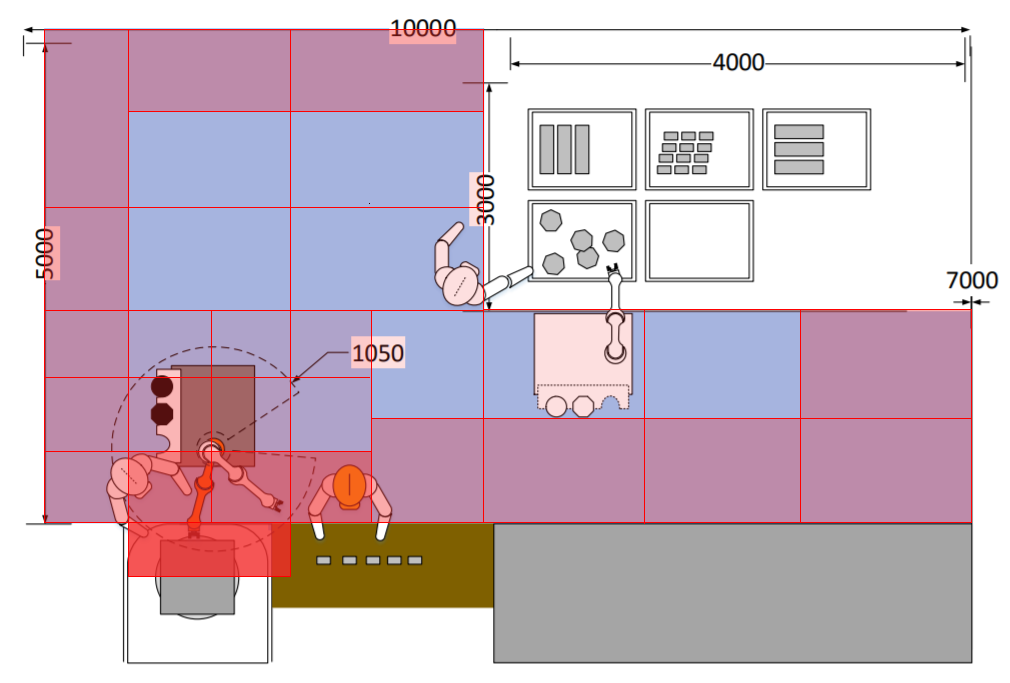
\includegraphics[width=\textwidth]{images/layout} 
% \caption{Subdivision of the layout, highlighted areas are the most dangerous ones} 
% \label{fig:layout} 
% \end{figure}

% \clearpage
% The most critical areas are the ones with indices from 1 to 12, particular attention must be paid to L\textsubscript0 too, since it is where the EE and O could be working together. 

% \begin{figure}[htp] 
% 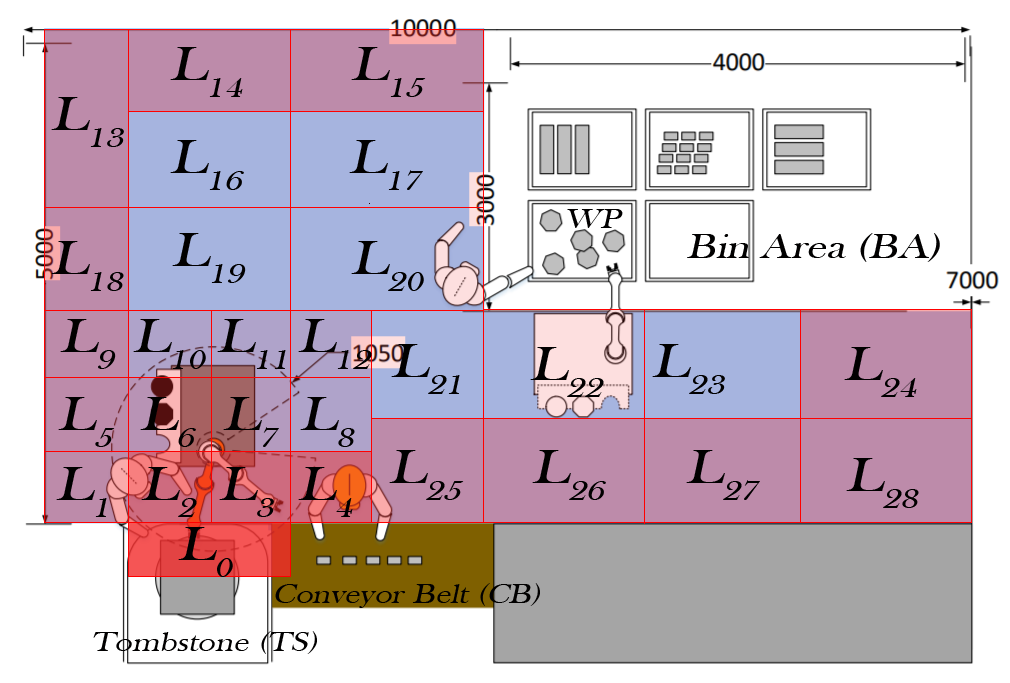
\includegraphics[width=\textwidth]{images/layoutnames} 
% \caption{Names of the splitted layout and various areas} 
% \label{fig:layout2} 
% \end{figure}


\subsubsection{Layout areas}
We discretized the layout in such a way that the most important and critical areas, in which Human-Robot interaction are very likely to happen, have a fine-grained grid, whereas the other areas, in which the Operator should not be present to assist the Robot, are modeled as bigger blocks in order not to introduce unnecessary complexity in the model and to avoid state space explosion.

The most critical areas are the ones with indices from 1 to 12, particular attention must be paid to L\textsubscript0 too, since it is where the EE and O could be working together. 

\begin{figure}[htp] 
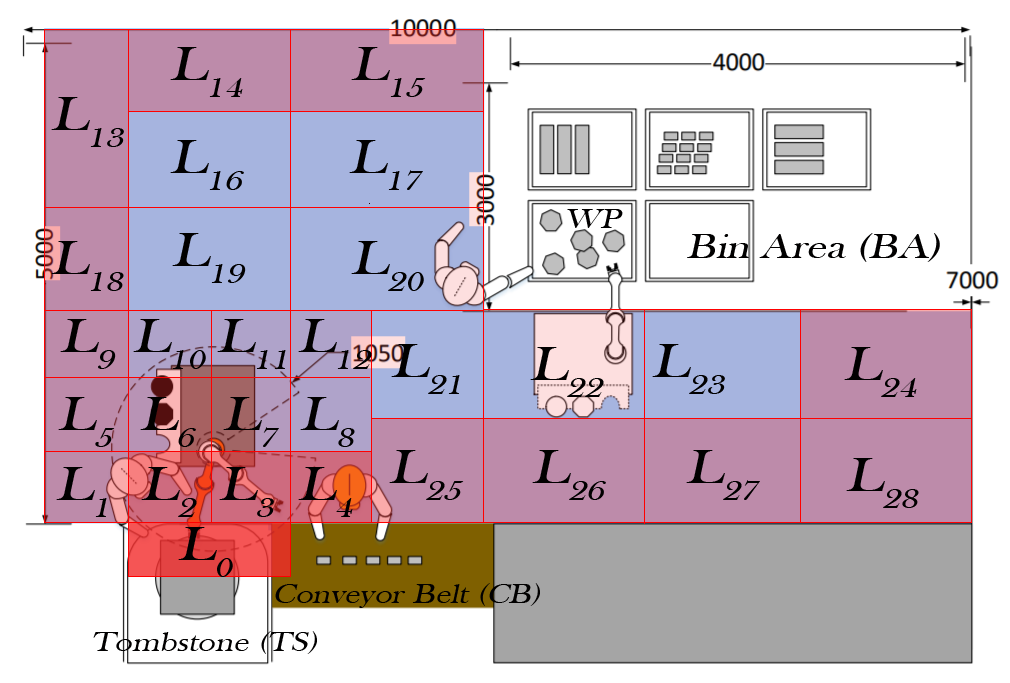
\includegraphics[width=0.9\textwidth]{images/layoutnames} 
\caption{Subdivision of the layout. The highligthed areas are the dangerous ones.} 
\label{fig:layout2} 
\end{figure}

\pagebreak
\subsection{Assumptions and modeling}
\paragraph{Robot}
The robot is discretized in two parts, the cart and the arm. The cart is such that it can only occupy one area at the time: this is a strong assumption, however it is vital because it reduces the complexity of our model. The arm is modeled by considering two joints and the end effector. The first joint is assumed to be the connection between the cart and the arm, therefore its position is at all times the same as the cart position. The second joint allows broader movement to the arm and it links the first joint to the end effector. The whole arm can reach at most a distance of two adjacent areas. The response of the actuators to a change in the control variables is assumed to be short enough to be modeled as instantaneous.

\paragraph{Human}
The human is discretized in body, head and arms. Each one of the parts can only occupy one area. The movement can only be observed, but not controlled, by the robot.

\paragraph{Bin Area}
We operated under the assumption that the Bin Area is always full, or better, it is never empty in any subarea of its space. With this assumption the KUKA robot will only have to stretch out from an adjacent area and pick as many WP as it wants without having to move to another adjacent area because there are no WP left where it is. 

\paragraph{Local Bin}
The local bin of R is where it stores the WPs in order to transport them from one place to the other. For the sake of simplicity we made as an assumption that the local bin can contain at most 3 pieces, so we could write formulae in a simple way, of course this can be generalized to N pieces in a trivial way.

\subsection{KUKA workflow}
The workflow of KUKA can be described by a FSA, we divided the tasks that R has to perform in 9 main elementary actions, whose formalization can be found in the \textbf{RobotController} TRIO+ class.
Those atomic actions whose name is self-explaining are:

\begin{enumerate}
    \item \textbf{PickFromBinArea}\@ 
    \item \textbf{DropToLocalBin}\@
    \item \textbf{GoToTombstone}\@ 
    \item \textbf{PickFromLocalBin}\@ 
    \item \textbf{DropToTombstone}\@ 
    \item \textbf{PickFromTombstone}\@ 
    \item \textbf{GoToConveyorBelt}\@ 
    \item \textbf{DropToConveyorBelt}\@ 
    \item \textbf{GoToBinArea}\@ 
\end{enumerate}
\clearpage
\subsection{Petri Net of KUKA workflow}
The following Petri net that represents the correct flow of actions that the robot has to perform.
\begin{center}
    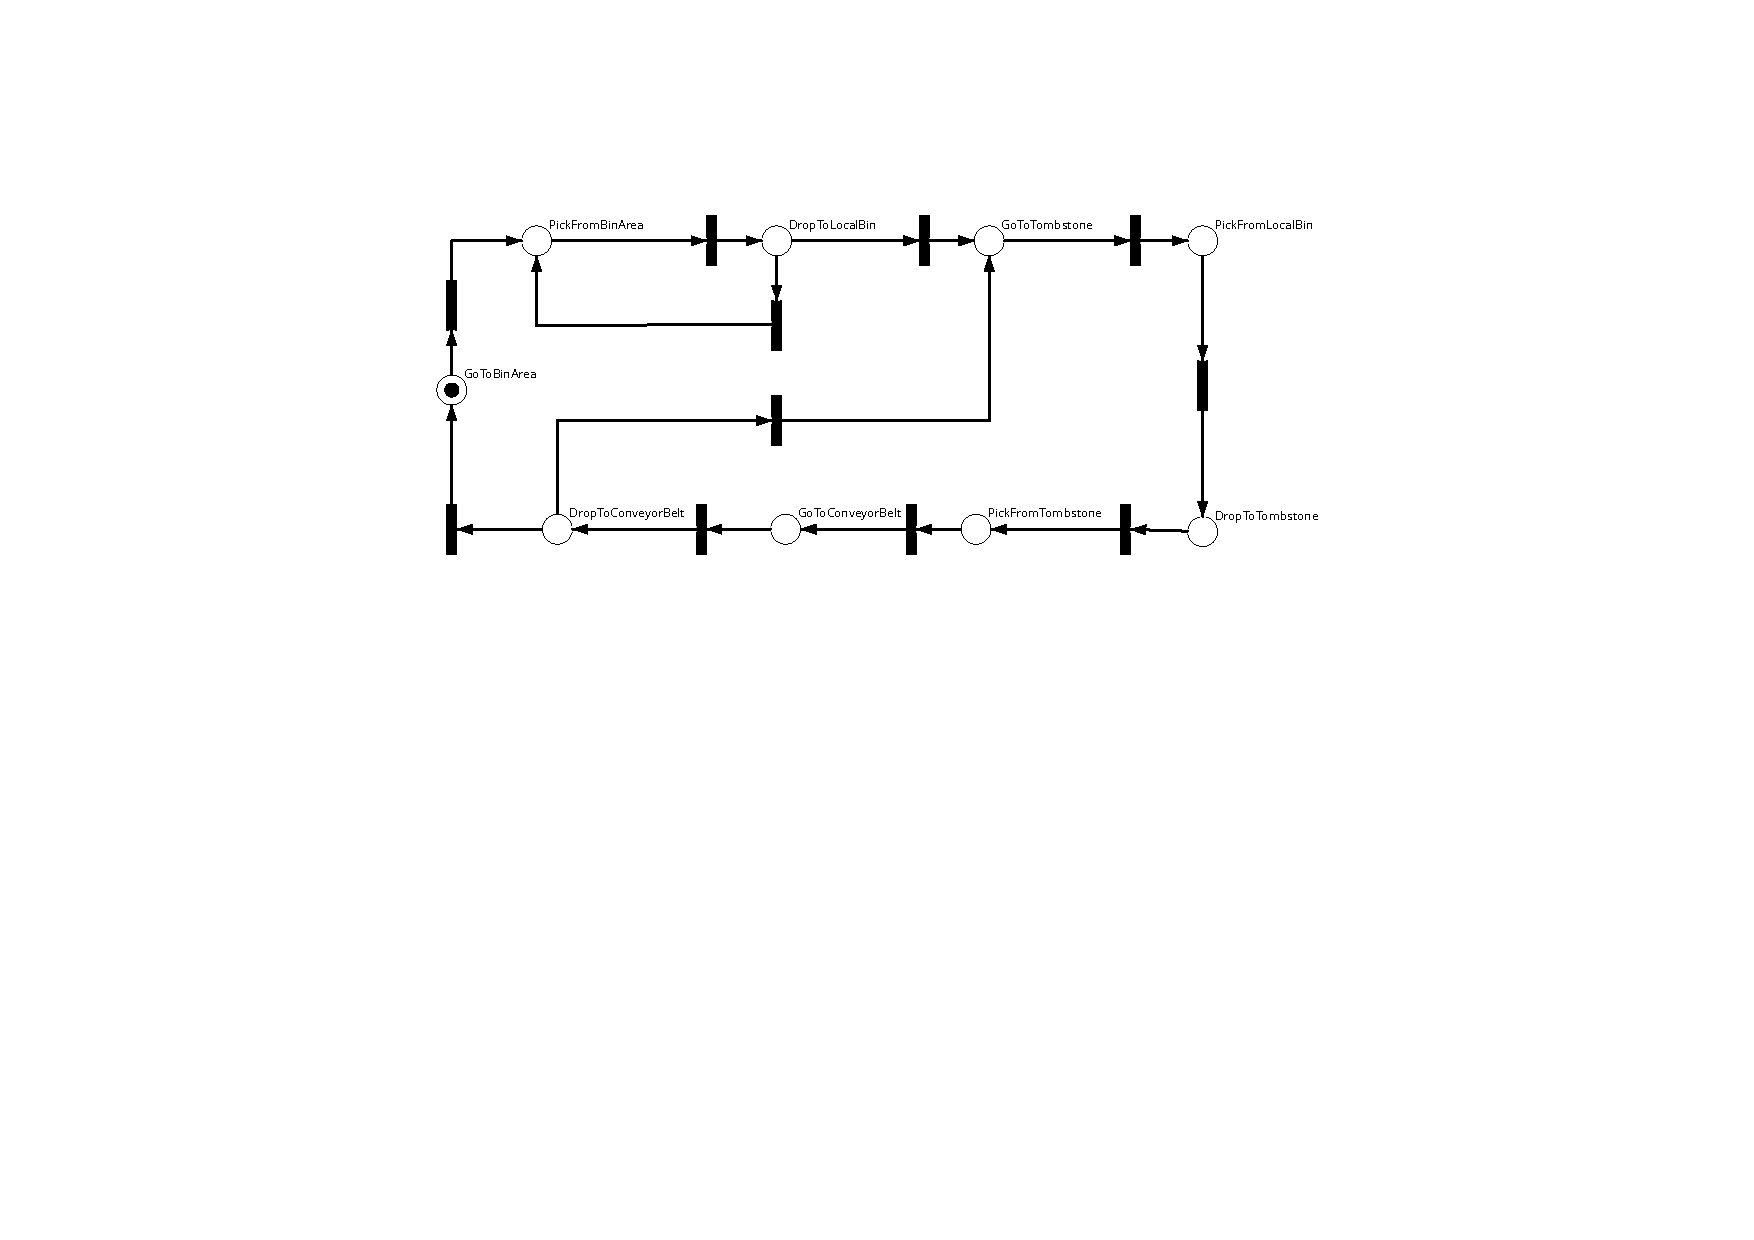
\includegraphics[width=18cm]{images/petriNetKuka}
\end{center}

\clearpage
\section{Archi-TRIO model}

\subsection{Class overview}
We organized the model in 12 TRIO+ classes, here we provide an overview of each one and a UML-like diagram to better visualize the connections among them.

\subsubsection{Grid}
The layout is discretized in this class, here we defined the adjacency predicate and the enumeration of subareas of L, as well as other specific predicates for special areas contained in L.

\subsubsection{Sensors}
The main superclass of sensors is \textbf{PositionSensor}, it uses as module the \textbf{Grid} and has 2 predicates: Position(layout area) and moved(), the subclasses which inherits them are the following ones:

\begin{itemize}
    \item \textbf{OperatorHeadPositionSensor}:\@ The sensor for the head of O
    \item \textbf{OperatorBodyPositionSensor}:\@ The sensor for the body of O
    \item \textbf{OperatorArmPositionSensor}:\@ The sensor for the arm of O
    \item \textbf{RobotArmPositionSensor}:\@
The sensor for the arm of O, in which the linkings and constraints are made consistent
    \item \textbf{RobotCartPositionSensor}:\@ The sensor for the Cart position in the layout
\end{itemize}

Then 2 main wrappers are created around the sensors, in which constraints among the various specific sensors are defined:
\begin{itemize}
    \item \textbf{OperatorPositionSensor}:\@ The wrapper sensor for O which imports as modules OperatorHeadPositionSensor, OperatorBodyPositionSensor, OperatorArmPositionSensor and the Grid
    \item \textbf{RobotPositionSensor}:\@ The wrapper sensor for R which imports as modules RobotArmPositionSensor, RobotCartPositionSensor and the Grid

\end{itemize}

\subsubsection{RobotStatus}
In this class we have the main predicates about the state of the robot and of its local bin (isFull, isEmpty), here we also define the targetCartSpeed and targetEESpeed which are the control variables, and currentCartSpeed, currentEESpeed which are read from sensors and defined as a part of the state of the robot itself.

\subsubsection{RobotController}
This is one of the most important classes, it handles all the actions performed by R, it specifies preconditions, axioms with constraints on what should be true while an action is being performed, and the actual sequence of events that the action is composed by.

\subsubsection{SafetyChecker}
Here we define all the constraints necessary for the safety of O in the presence of a working KUKA R around the layout, all the actions performed by R that could cause harm to O are avoided or limited as much as possible.

\subsection{UML diagram}
This diagram shows the connections and hierarchies among classes.
\begin{center}
    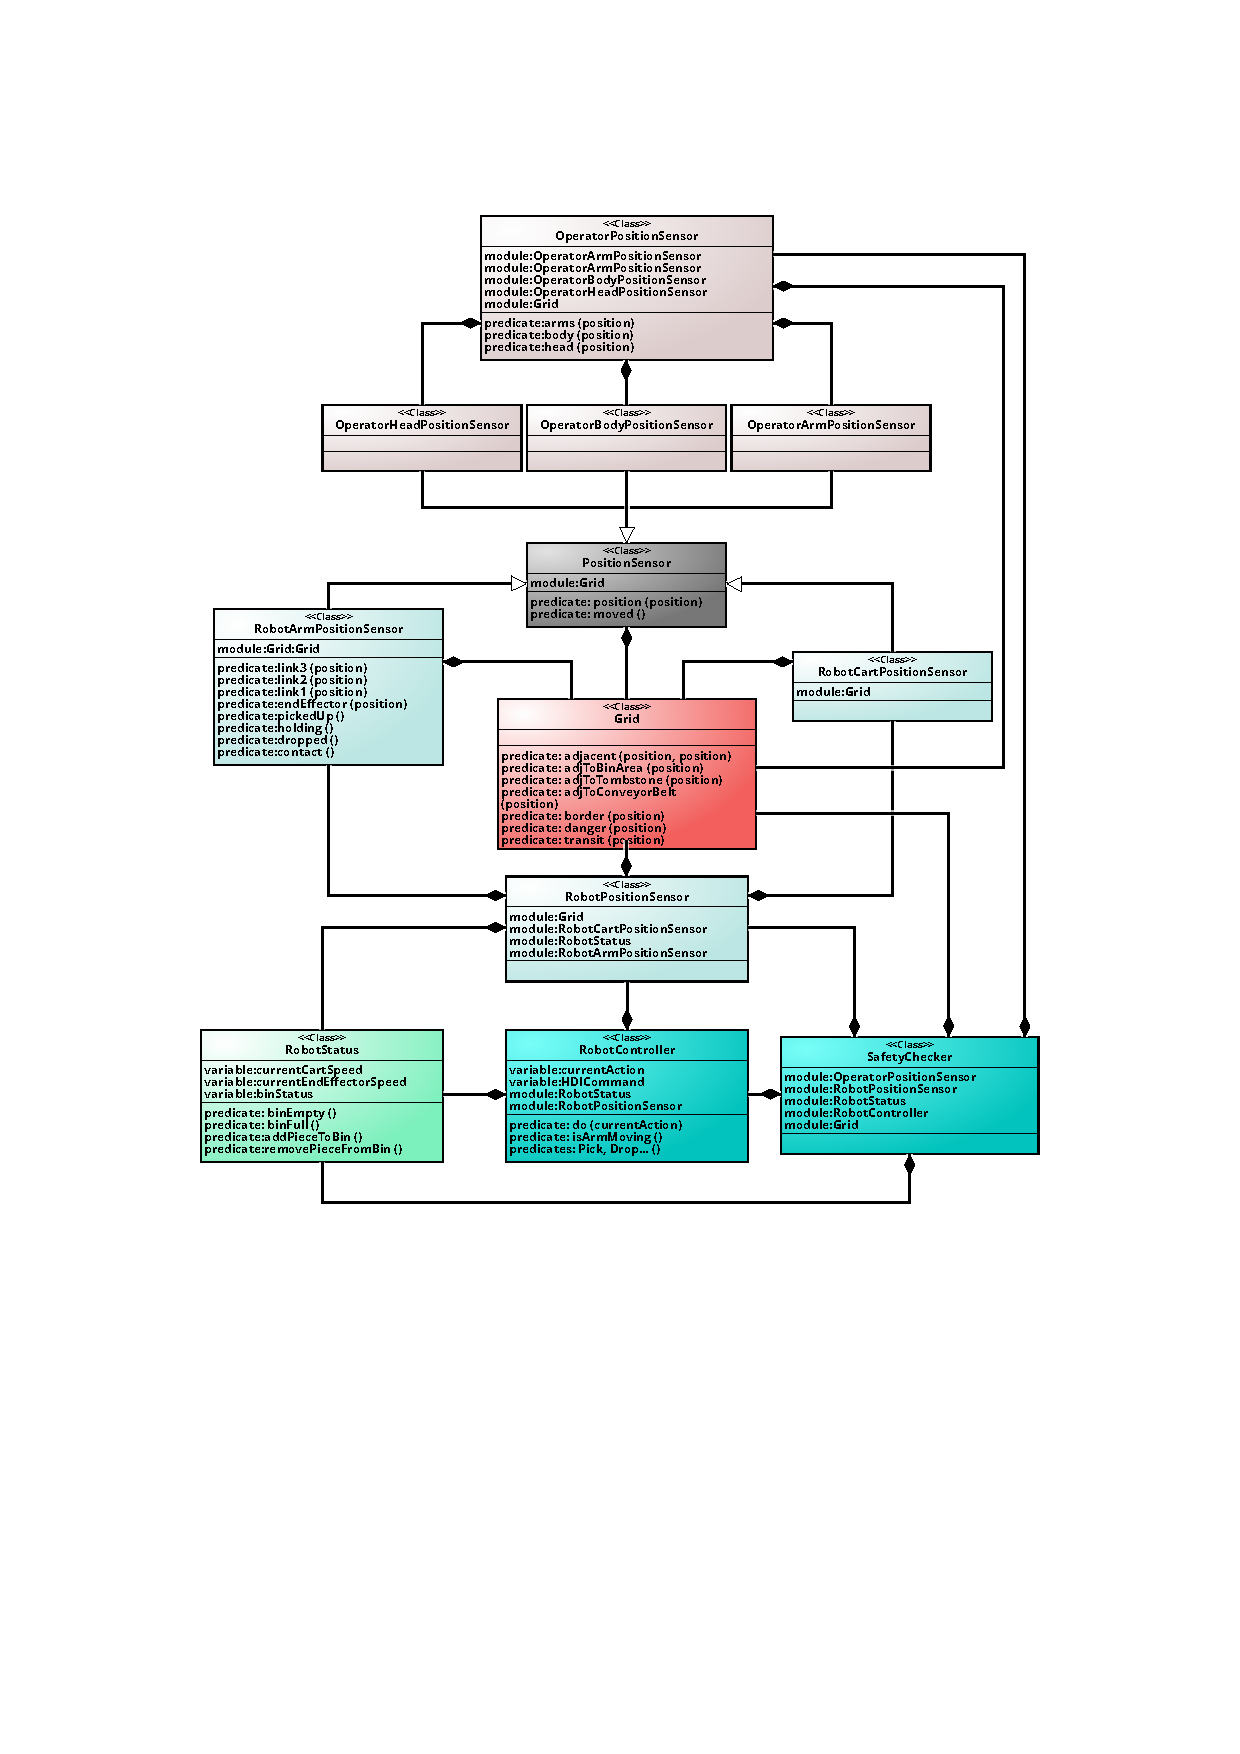
\includegraphics[width=16.5cm]{images/ArchiTRIO}
\end{center}
\clearpage
\section{TRIO+ specification}

\subsection{Definition of Grid class}
\begin{lstlisting}[fontadjust, mathescape, frame=single] 
class Grid
    visible adjacent;

    temporal domain integer;

    TI items
        predicates 
                    adjacent(position, position);
                    
                    adjToBinArea({ L0, L1, L2, L3, L4, L5, L6, L7, L8, L9,
                            L10, L11, L12, L13, L14, L15, L16, L17, L18, L19,
                            L20, L21, L22, L23, L24, L25, L26, L27, L28, LBA, LCB}),
                    adjToTombstone({ L0, L1, L2, L3, L4, L5, L6, L7, L8, L9,
                            L10, L11, L12, L13, L14, L15, L16, L17, L18, L19,
                            L20, L21, L22, L23, L24, L25, L26, L27, L28, LBA, LCB}),
                    adjToConveyorBelt({ L0, L1, L2, L3, L4, L5, L6, L7, L8, L9,
                            L10, L11, L12, L13, L14, L15, L16, L17, L18, L19,
                            L20, L21, L22, L23, L24, L25, L26, L27, L28, LBA, LCB}),
                    border({ L0, L1, L2, L3, L4, L5, L6, L7, L8, L9,
                            L10, L11, L12, L13, L14, L15, L16, L17, L18, L19,
                            L20, L21, L22, L23, L24, L25, L26, L27, L28, LBA, LCB}),
                    danger({ L0, L1, L2, L3, L4, L5, L6, L7, L8, L9,
                            L10, L11, L12, L13, L14, L15, L16, L17, L18, L19,
                            L20, L21, L22, L23, L24, L25, L26, L27, L28, LBA, LCB}),
                    transit({ L0, L1, L2, L3, L4, L5, L6, L7, L8, L9,
                            L10, L11, L12, L13, L14, L15, L16, L17, L18, L19,
                            L20, L21, L22, L23, L24, L25, L26, L27, L28, LBA, LCB}),

    axioms
        
        -- This is the formula that appears into the document's appendix.
        -- Specifies which areas are adjacent one with another
        adjacency:$ 
            \forall x, y (adjacent(x,y) -> ... );$

        dangerArea:$
            danger(L0) \land danger(L2) \land danger(L3) \land danger(L4) \land danger(L6) \land danger(L7) \land danger(L8) \land danger(L10) \land danger(L11) \land danger(L12) \land 
            danger(L15) \land danger(L17) \land danger(L20) \land danger(L22) \land danger(L23) \land danger(L24) \land 
            \neg danger(L1) \land \neg danger(L5) \land \neg danger(L9) \land \neg danger(L13) \land \neg danger(L14) \land \neg danger(L16) \land \neg danger(L18) \land
            \neg danger(L19) \land \neg danger(L21) \land \neg danger(L25) \land \neg danger(L26) \land \neg danger(L27) \land \neg danger(L28);$
        
        borderArea:$
            border(L1) \land border(L2) \land border(L3) \land border(L4) \land border(L25) \land border(L26) \land border(L27) \land border(L28) \land border(L24) \land border(L23) \land border(L22) \land border(L20) \land border(L17) \land border(L15) \land border(L14) \land border(L13) \land border(L18) \land border(L9) \land border(L5) \land 
            \neg border(L0) \land \neg border(L6) \land \neg border(L7) \land \neg border(L8) \land \neg border(L10) \land \neg border(L11) \land \neg border(L12) \land \neg border(L21) \land \neg border(L16) \land \neg border(L19);$

        transitArea:$
            \forall x (transit(x) \iff \neg border(x) || \neg danger(x) );$

        binArea:$
            \forall x (adjToBinArea(x) \iff adjacent(x, LBA);$

        tombstone:$
            \forall x (adjToTombstone(x) \iff adjacent(x, L0);$

        conveyorBelt:$
            \forall x (adjToConveyorBelt(x) \iff adjacent(x, LCB);$
end Grid.\end{lstlisting}

\pagebreak
\subsection{Definition of the PositionSensor class}
\begin{lstlisting}[fontadjust, mathescape, frame=single]
    
-- This is the basic sensor of our system. Allows to define a predicate position,
-- that will be used by the robot's position sensors.   
class PositionSensor
    visible position, adjacent;

    temporal domain integer;

    -- The domain of the predicate position lies inside all the possible areas
    -- of interest. 
    -- The predicate moved allows us to manage the robot's movement. This is due
    -- to the fact that the robot can move at three speed intensity. Therefore, 
    -- for a correct modelization of this movement, we needed a predicate that 
    -- tell us whether the robot has moved in this time instant.
    TD items 
        predicates  position({L0, L1, L2, L3, L4, L5, L6, L7,
                              L8, L9, L10, L11, L12, L13, L14,
                              L15, L16, L17, L18, L19, L20, L21,
                              L22, L23, L24, L25, L26, L27, L28,
                              LBA, LCB});
                    moved();

    modules: Grid: Grid;

    connection: {(Grid.adjacent, adjacent)};

    axioms
        moved:$ moved() \iff \exists x \past(position(x), 1) \land \neg position(x);$

end PositionSensor.\end{lstlisting}

\pagebreak
\subsection{Definition of the operator's sensor classes}
\begin{lstlisting}[fontadjust, mathescape, frame=single] 
-- Simple class that specify the predicates for the position of
-- the operator's arm. The arm can be in only one position in 
-- the map at each time instant. 
-- One thing to notice is that in our model the operator will have
-- two arms.

class OperatorArmPositionSensor
    inherits PositionSensor

    visible position;

    temporal domain integer;

    axioms
        -- the arm always exists
        existsArm: $\exists x (position(x));$

        -- the arm is only in one area
        uniqueArm: $\forall x (position(x) \implies \nexists y (position(y) \land x \neq y));$

end OperatorArmPositionSensor.
\end{lstlisting}
\begin{lstlisting}[fontadjust, mathescape, frame=single] 
-- Simple class that specify the predicate position for the 
-- operator's body. The body can be in only one position at
-- each time instant.

class OperatorBodyPositionSensor
    inherits PositionSensor

    visible position;

    temporal domain integer;

    axioms
        -- the body is only in one area
        uniqueBody: $\forall x (position(x) \implies \nexists y (position(y) \land x \neq y));$

end OperatorBodyPositionSensor.
\end{lstlisting}
\pagebreak
\begin{lstlisting}[fontadjust, mathescape, frame=single] 
-- This class defines the position that the head of the
-- operator assumes at each time instant. This position
-- will be crucial for the definition of the safety 
-- properties. 
-- We assume also that the head of hhe operator can be in
-- only one position at each time instant.

class OperatorHeadPositionSensor
    inherits PositionSensor
    
    visible position;

    temporal domain integer;

    TODO: conformare questa formula come le formule sopra per mantenere lo 
    TODO: stesso formato

    axioms
        -- The head can be only in one area at each time
        headIsUnique: $\exists x (position(x) \land \forall y (y \neq x \implies \neg position(y)));$

end OperatorHeadPositionSensor.
\end{lstlisting}
\begin{lstlisting}[fontadjust, mathescape, frame=tlb] 
class OperatorPositionSensor
    inherits PositionSensor
    visible arms, body, head;$

    temporal domain integer;$

    TD items
        predicates
            arms({L0, L1, L2, L3, L4, L5, L6, L7, L8, L9,
                      L10, L11, L12, L13, L14, L15, L16, L17, L18, L19,
                      L20, L21, L22, L23, L24, L25, L26, L27, L28 }),
            body({L0, L1, L2, L3, L4, L5, L6, L7, L8, L9,
                      L10, L11, L12, L13, L14, L15, L16, L17, L18, L19,
                      L20, L21, L22, L23, L24, L25, L26, L27, L28 }),
            head({L0, L1, L2, L3, L4, L5, L6, L7, L8, L9,
                      L10, L11, L12, L13, L14, L15, L16, L17, L18, L19,
                      L20, L21, L22, L23, L24, L25, L26, L27, L28 });$


    modules LeftArm:$ OperatorArmPositionSensor,
            RightArm:$ OperatorArmPositionSensor,
            Body:$ OperatorBodyPositionSensor,
            Head:$ OperatorHeadPositionSensor,
            Grid:$ Grid;$

    axioms
        -- connect the predicates between the modules
        arms:$ \forall x (arms(x) \iff (LeftArm.position(x) || RightArm.position(x)));$
        body:$ \forall x (body(x) \iff Body.position(x));$
        head:$ \forall x (head(x) \iff Head.position(x));$

        -- head is on the body or in a close by cell
        headOnTheBody:$ \forall x (head(x) \limply body(x) || \exists y (body(y) \land Grid.adjacent(x, y)));$

        -- arms are on the body or in a close by cell
        armsOnTheBody:$ \forall x (arms(x) \limply body(x) || \exists y (body(y) \land Grid.adjacent(x, y)));$

        -- the operator can move one area in each time instant
        movement:$ \forall x (body(x) \limply \exists y (\  future(body(y), 1) \land (x == y || Grid.adjacent(x, y))));$
end OperatorPositionSensor.\end{lstlisting}

\pagebreak
\subsection{Definition of the robot's sensor classes}
\begin{lstlisting}[fontadjust, mathescape, frame=single] 
-- This class specify the sensors for the robot's arm. We decide
-- to model the arm as the real one present on the KUKA unit.
-- The arm is composed of 3 links and one end effector.
-- There are three predicates that will be use to determine
-- when the robot is switching between an action an another,
-- and they are pickedUp(), holding() and dropped().

class RobotArmPositionSensor
    inherits PositionSensor

    temporal domain integer;

    visible position, link3, link2, endEffector, pickedUp, holding, dropped;

    modules Grid: Grid;

    TD items
        predicates
            -- Link3 is the first segment of the arm from the body of the robot
            link3({ L0, L1, L2, L3, L4, L5, L6, L7, L8, L9,
                    L10, L11, L12, L13, L14, L15, L16, L17,
                    L18, L19, L20, L21, L22, L23, L24, L25,
                    L26, L27, L28, LBA, LCB}),
                    
            -- Link2 is the second segment of the arm, linked to link3 and link1
            link2({ L0, L1, L2, L3, L4, L5, L6, L7, L8, L9,
                    L10, L11, L12, L13, L14, L15, L16, L17,
                    L18, L19, L20, L21, L22, L23, L24, L25,
                    L26, L27, L28, LBA, LCB}),
                    
            -- Link1 is the third segment of the arm, which is the end effector 
            link1({ L0, L1, L2, L3, L4, L5, L6, L7, L8, L9,
                    L10, L11, L12, L13, L14, L15, L16, L17,
                    L18, L19, L20, L21, L22, L23, L24, L25,
                    L26, L27, L28, LBA, LCB}),
                     
            -- same as link1, used for clarity
            endEffector({ L0, L1, L2, L3, L4, L5, L6, L7, L8, L9,
                          L10, L11, L12, L13, L14, L15, L16, L17,
                          L18, L19, L20, L21, L22, L23, L24, L25,
                          L26, L27, L28, LBA, LCB}),
                    

            -- Signal if the pick action has been completed successfully
            pickedUp(),

            
            -- Signal to model the fact that the robot is holding a piece
            holding(),

            -- Signal to model the fact that the robot has dropped the piece it
            -- was holding
            dropped();

            -- Signal to model the fact that the robot's arm is being touched by
            -- the operator
            contact();

    axioms:

        -- The position is all the cells that are occupied by the arm
        armPosition: 
            $\forall x (position(x) \iff link2(x) \lor link1(x));$
        
        -- link 2 is connected to link3
        connection32: 
            $\forall x \forall y (link2(x) \implies$
                 $link3(x) \lor (x \neq y \land link3(y) \land Grid.adjacent(x, y)));$

        -- link1 is connected to link2
        connection21: 
            $\forall x \forall y (link1(x) \implies$ 
                 $link2(x) \lor (x \neq y \land link2(y) \land Grid.adjacent(x, y)));$

        -- end effector is link1
        endEffectorOnLink1:
            $\forall x (endEffector(x) \iff link1(x));$

        -- the link1 always exists
        existsLink1: $\exists x (link1(x));$

        -- the link1 is only in one area
        uniqueLink1: $\forall x (link1(x) \implies \nexists y (link1(y) \land x \neq y));$
        
        -- the link2 always exists
        existsLink2: $\exists x (link2(x));$

        -- the link2 is only in one area
        uniqueLink2: $\forall x (link2(x) \implies \nexists y (link2(y) \land x \neq y));$

        -- the link3 always exists
        existsLink3: $\exists x (link3(x));$

        -- the link3 is only in one area
        uniqueLink3: $\forall x (link3(x) \implies \nexists y (link3(y) \land x \neq y));$    

        -- the arm cannot teleport
        armCannotTeleport:
            $\forall x (endEffector(x) \implies$ 
                $(\future (endEffector(x) \lor (\exists y (endEffector(y) \land Grid.adjacent(x,y))), 1)))$;

        -- Only one of pickedUp(), holding() and dropped() can be true in 
        -- each instant
        onlyOne:
            $(pickedUp() \implies$
                $\neg holding() \land \neg dropped()) \land$
            $(holding() \implies$ 
                $\neg pickedUp() \land \neg dropped()) \land$
            $(dropped() \implies$
                $\neg pickedUp() \land \neg holding());$

        -- holding() holds between pickedUp() and dropped()
        sequence:
            $\becomes(\neg pickedUp()) \land \until(holding(), dropped());$

end RobotArmPositionSensor.
\end{lstlisting}
\begin{lstlisting}[fontadjust, mathescape, frame=single] 
-- The robot has a position, and from that position it can be present only in
-- Grid.adjacent areas from the position. The Position predicate represent these adjacent
-- position, while the position predicate specify the current central position of the robot.
-- Another condition we need to supply is the fact that the robot cannot "teleport".
-- This condition is guaranteed by the fact that any new position that the robot assumes
-- must be Grid.adjacent to at least one position of the robot in the past.

class RobotCartPositionSensor;
    inherits PositionSensor
    
    visible position, moved;
    
    temporal domain integer;

    modules Grid: Grid;
    
    axioms
    
        -- The position is unique
        positionUnique:$ 
            \forall x (position(x) \limply (\forall y (y != x \limply \neg position(y))));$          

        -- An area occupied by the robot must be Grid.adjacent with an area occupied by the robot in the past
        do\lnotTeleport:$
            \forall x (\becomes(position(x)) \limply \exists y (\past(position(y), 1) \land Grid.adjacent(x, y)));$
            
end RobotCartPositionSensor.\end{lstlisting}
\pagebreak
\begin{lstlisting}[fontadjust, mathescape, frame=single] 
-- This is the class that collects all the sensor of the
-- robot.
-- In this class we defined a predicate for the robot's velocities,
-- both for the arm and the cart. We defined axioms to check the
-- robot's movement. As example, if the robot is moving at low speed,
-- it can move in a adjacent area in two time unit. This modelization
-- is permitted through the use of a support predicate moved().
-- We also define a predicate contact to model the fact that the robot's
-- arm can be touched by the operator to guide its working process.
-- Some specific axioms has been defined to model the situation
-- explained before.

class RobotPositionSensor
    temporal domain integer

    visible Cart, Arm;

    modules Cart: RobotCartPositionSensor,
             Arm: RobotArmPositionSensor,
             Status: RobotStatus,
             Grid: Grid;

    axioms
        -- link3 is in the same position as the cart
        link3OnCart: 
            $\forall x (Arm.link3(x) \iff Body.position(x));$

        -- cartTargetSpeed defines how often the robot cart can move in the grid
        cartSpeedNone: 
            $Status.currentCartSpeed == None \implies$ 
                $\exists x \future(Cart.position(x), 1) \land Cart.position(x);$

                
        cartSpeedLowMoved: 
            $\exists x (Status.currentCartSpeed == Low \land Cart.moved() \implies$
                $Cart.position(x) \land \future(Cart.position(x), 1));$

        cartSpeedLowNotMoved: 
            $\exists x (Status.currentCartSpeed == Low \land \neg Cart.moved() \implies$
                $Cart.position(x) \land \exists y (\future(Cart.position(y), 1) \land x \neq y \land Grid.adjacent(x, y)));$

        cartSpeedNormal: 
            $\exists x (Status.currentCartSpeed == Normal \land Cart.position(x) \implies$
                $\exists y (\future(Cart.position(y), 1) \land x \neq y \land Grid.adjacent(x, y)));$




        -- if the speed is low, then the arm can move from one area to another
        -- only half of the time
        armSpeedLowMoved: 
            $\exists x (Status.currentCartSpeed == None \land Status.currentArmSpeed == Low \land$
              $Arm.moved() \implies$ 
                  $Arm.endEffector(x) \land \future(Arm.endEffector(x), 1));$

        armSpeedLowNotMoved: 
            $\exists x (Status.currentCartSpeed == None \land Status.currentArmSpeed == Low \land$ 
            $\past(\neg Arm.moved() \land Arm.endEffector(x), 1) \implies$ 
                $Arm.endEffector(y) \land x \neq y \land Grid.adjacent(x, y)));$

        -- if the speed is normal, then the arm can move from one area to 
        -- another at every time instant
        armSpeedNormal: 
            $\exists x (Status.currentCartSpeed == None \land$
              $Status.currentArmSpeed == Normal \land$
              $Arm.endEffector(x) \implies$
                  $\exists y (\future(Arm.endEffector(y), 1) \land x \neq y \land Grid.adjacent(x, y)));$

        -- if the cart is moving, then the arm must stay on top of the cart,
        -- both the end effector and the link
        armOnTopMovingCart: 
            $\forall x (Status.currentCartSpeed \neq None \land Cart.moved() \land Cart.position(x) \implies$
                $Arm.position(x));$


        --------------------
        -- CONTACT AXIOMS --
        --------------------

        -- the Arm.contact() predicate can be true only when the arms of the 
        -- operator are in the same area as the arm of the robot
        armContact:
            $\forall x (Arm.position(x) \land Arm.contact() \implies$
                $Operator.arms(x));$

        -- when the operator is touching the arm of the robot, the speed of the
        -- arm of the robot is none
        stoppedWhileContact:
            $Arm.contact() \implies $
                $RobotStatus.currentEndEffectorSpeed == None;$






                
        -- if the operator is moving the end effector, then the end effector 
        -- will move even if the speed is none
        armSpeedNoneWithContact: 
            $\forall x(Status.currentArmSpeed == None \land Arm.contact() \land Arm.endEffector(x)\implies$
                $\exists y \future(Arm.endEffector(y) \land (x == y \lor Grid.adjacent(x, y)), 1));$
        
end RobotPositionSensor.
\end{lstlisting}

\pagebreak
\subsection{Definition of the state of the robot}
\begin{lstlisting}[fontadjust, mathescape, frame=tlb] 
class RobotStatus

  temporal domain integer;$

  visible targetCartSpeed, targetEndEffectorSpeed, binEmpty, binFull, addPieceToBin, removePieceFromBin, currentCartSpeed, currentEndEffectorSpeed;$

  TD items:$
  predicates
    binEmpty(),
    binFull(),
    addPieceToBin(),
    removePieceFromBin();$

  vars
    targetCartSpeed({None, Low, Normal}),
    currentCartSpeed({None, Low, Normal}),
    targetEndEffectorSpeed({None, Low, Normal}),
    currentEndEffectorSpeed({None, Low, Normal}),
    binStatus({Empty, 1, 2, Full});$

  axioms

  -- bin empty
  binEmpty() \iff binStatus == Empty;$

  -- bin full
  binFull() \iff binStatus == Full;$

  -- ordering of bin status
  binStatus == Empty \land addPieceToBin() \limply \exists x (\becomes(binStatus == 1, x));$
  binStatus == 1 \land addPieceToBin() \limply \exists x (\becomes(binStatus == 2, x));$
  binStatus == 2 \land addPieceToBin() \limply \exists x (\becomes(binStatus == Full, x));$
  binStatus == Full \land removePieceFromBin() \limply \exists x (\becomes(binStatus == 2, x));$
  binStatus == 2 \land removePieceFromBin() \limply \exists x (\becomes(binStatus == 1, x));$
  binStatus == 1 \land removePieceFromBin() \limply \exists x (\becomes(binStatus == Empty, x));$

  -- a piece can be added to the local bin only if there is enough capacity
  addPieceToBin() \limply \neg binStatus == Full;$

  -- a piece can be removed from the local bin only if there is at least one in the bin
  removePieceFromBin() \limply \neg binStatus == Empty;$

  -- addPieceToBin() and removePieceFromBin() are instantaneous events
  singleInstantEvents:$
  (addPieceToBin() \limply \  future(\neg addPieceToBin(), 1));$
  (removePieceFromBin() \limply \  future(\neg removePieceFromBin(), 1));$

  -- binStatus stays constant if there is no action performed
  constantBin:$ \forall x (binStatus == x \land \neg (addPieceToBin() || removePieceFromBin()) \limply \  future(binStatus == x, 1));$

end RobotStatus.\end{lstlisting}

\pagebreak
\subsection{Definition of the RobotController class}
\begin{lstlisting}[fontadjust, mathescape, frame=single]
class RobotController
  -- RobotController handles all the actions that the robot can execute, 
  -- specifying preconditions, axioms over the duration of the action
  -- and the sequences of events that must happen during the action

  temporal domain integer;

  TD items

  predicates
    do({
    PickFromBinArea,
    DropToLocalBin,
    GoToTombstone,
    PickFromLocalBin,
    DropToTombstone,
    PickFromTombstone,
    GoToConveyorBelt,
    DropToConveyorBelt,
    GoToBinArea
    });

    isArmMoving(),
    PickFromBinAreaT0(), PickFromBinAreaT1(),
    PickFromBinAreaT2(), PickFromBinAreaT3();

  variables
    currentAction({
    PickFromBinArea,
    DropToLocalBin,
    GoToTombstone,
    PickFromLocalBin,
    DropToTombstone,
    PickFromTombstone,
    GoToConveyorBelt,
    DropToConveyorBelt,
    GoToBinArea
    }),

    -- None -> Proceed normally with the execution
    -- Emergency -> Stop the robot and wait for the HDICommand to return to None
    -- Continue -> when the robot has placed a piece on the tombstone, it needs 
    -- to wait for the lavoration to be done and for the operator to signal that 
    -- the lavoration has terminated.

    HDICommand({
    None,
    Emergency,
    Continue
    });
    
  TI items 
  
  consts MaxDropTime: integer,
       MaxPickUpTime: integer,
       MaxTravelTime: integer;

  modules RobotStatus: RobotStatus,
                Robot: RobotPositionSensor;

  
  
  axioms

  -- CORRECT FLOW OF ACTIONS

    -- the actions must be done in the correct order
    correctActionOrder:
      $(currentAction == PickFromBinArea \limply $
        $\until(currentAction == PickFromBinArea, currentAction == DropToLocalBin))
      \ \land$

      -- After having dropped a piece in the local bin, the robot either takes 
      -- another or goes to the tombstone
      $(currentAction == DropToLocalBin \limply $
        $(\until(currentAction == DropToLocalBin,currentAction == PickFromBinArea)\ ||$
        $\until(currentAction == DropToLocalBin, currentAction == GoToTombstone)))
      \ \land$

      -- After having gone to the tombstone, the robot takes the stored working 
      -- piece with the end effector
      $(currentAction == GoToTombstone \limply $
        $(\until(currentAction == GoToTombstone, currentAction == PickFromLocalBin)))
      \ \land$

      -- After having picked up a piece from the local bin, the robot drops it 
      -- into the tombstone
      $(currentAction == PickFromLocalBin \limply $
        $\until(currentAction == PickFromLocalBin, currentAction == DropToTombstone))
      \ \land$

      -- After having dropped a piece into the tombstone, the robot waits for  
      -- the operator's signal and then picks up the reshaped piece
      $(currentAction == DropToTombstone \limply $ 
        $\until(currentAction == DropToTombstone, currentAction = PickFromTombstone))
      \ \land$

      -- After having picked up the piece from the tombstone, the robot goes to
      -- the conveyor belt
      $(currentAction == PickFromTombstone \limply $
        $\until(currentAction == PickFromTombstone, currentAction = GoToConveyorBelt))
      \ \land$


      -- After having gone to the conveyor belt, the robot drops the piece onto
      -- it
      $(currentAction == GoToConveyorBelt \limply $
        $\until(currentAction == GoToConveyorBelt, currentAction == DropToConveyorBelt)
      \ \land$

      -- After having dropped the piece onto the conveyor belt, the robot either 
      -- goes back to the tombstone or it goes to the bin area if local bin is 
      -- empty
      $(currentAction == DropToConveyorBelt \limply $
        $\until(currentAction == DropToConveyorBelt, currentAction == GoToTombstone)\ ||$
        $\until(currentAction == DropToConveyorBelt, currentAction == GoToBinArea))
      \ \land$

      -- After having gone to the bin area, the robot picks up a piece from the 
      -- bin area
      $(currentAction == GoToBinArea \limply $
        $\until(currentAction == GoToBinArea, currentAction == PickFromBinArea);$

    -- the change in currentAction must be preceded by a do request
    correctInit:
      $\forall x (\becomes(currentAction == x) \iff do(x));$

    
    -- during emergency mode, the robot needs to be stopped immediately
    emergencyMode:
      $(HDICommand == Emergency) \limply $
        $(RobotStatus.TargetCartSpeed == None) \land (RobotStatus.TargetEndEffectorSpeed == None);$

    -- do is an instantaneous event (lasts only one time instant)
    instantaneousDo:
        $\forall x (do(x) \limply \future(\neg do(x), 1));$

  -- DEFINITION OF PRECONDITIONS, AXIOMS HOLDING DURING THE ACTION 
  -- AND SEQUENCES OF EVENTS

  -- PickFromBinArea
    -- the robot has space in the local bin and is at the bin area
    prePickFromBinArea:
        $\becomes(currentAction == PickFromBinArea) \limply$
            $\neg RobotStatus.binFull() \land \neg Robot.Arm.holding() \land$
            $\forall x (Robot.Cart.position(x) \limply Grid.adjToBinArea(x));$

    -- the robot must be still
    duringPickFromBinArea:
        $currentAction == PickFromBinArea \limply RobotStatus.currentCartSpeed == None;$

    
    -- t0: Start -> end effector on top of cart, not holding
    -- t1: end effector on top of bin area, not holding
    -- t2: end effector on top of bin area, holding
    -- t3: End -> end effector on top of cart, holding
    $PickFromBinAreaT0() \iff (currentAction == PickFromBinArea \land \neg Robot.Arm.holding() \land$
        $\exists x (Robot.Cart.position(x) \land Robot.Arm.endEffector(x)))$;
    
    $PickFromBinAreaT1() \iff (currentAction == PickFromBinArea \land \neg Robot.Arm.holding() \land$
        $Robot.Arm.endEffector(LBA)))$;
    
    $PickFromBinAreaT2() \iff (currentAction == PickFromBinArea \land Robot.Arm.holding() \land$
        $Robot.Arm.endEffector(LBA)))$;
    
    $PickFromBinAreaT3() \iff (currentAction == PickFromBinArea \land Robot.Arm.holding() \land$
        $\exists x (Robot.Cart.position(x) \land Robot.Arm.endEffector(x)))$;
    
    -- to complete the PickFromBinArea action we need to have reached
    -- PickFromBinAreaT3()
    $\becomes(\neg currentAction == PickFromBinArea) \implies Past(PickFromBinAreaT3(), 1)$;
    
    -- from T3 to T2 the only thing that changes is the position
    -- of the end effector
    $PickFromBinAreaT3() \implies \exists t (\lasttime(PickFromBinAreaT2(), t) \land$
        $\lastedOp_{ie}(currentAction == PickFromBinArea \land Robot.Arm.holding(), t))$;

    -- from T2 to T1 the only thing that changes is the fact that
    -- the end effector is holding a piece
    $PickFromBinAreaT2() \implies \exists t (\lasttime(PickFromBinAreaT1(), t) \land$
        $\lastedOp_{ie}(currentAction == PickFromBinArea \land Robot.Arm.endEffector(LBA)))$;
    
    -- from T1 to T0 the only thing that changes is the position
    -- of the end effector
    $PickFromBinAreaT1() \implies \exists t (\lasttime(PickFromBinAreaT0(), t) \land$
        $\lastedOp_{ie}(currentAction == PickFromBinArea \land \neg Robot.Arm.holding()))$;
      
  -- DropToLocalBin
    -- the robot holds a piece, the local bin isn't full and the endEffector 
    -- is on the cart
    preDropToLocalBin:
        $\becomes(currentAction == DropToLocalBin) \limply $
            $\neg RobotStatus.binFull() \land Robot.Arm.holding() \land $
            $\exists x (Robot.Cart.position(x) \land \textit{Robot.Arm.endEffector}(x));$
    
    -- the robot cannot move, the endEffector must stay in the same zone
    duringDropToLocalBin:
        $currentAction == DropToLocalBin \limply $
            $(RobotStatus.currentCartSpeed == None \land$
            $RobotStatus.currentEndEffectorSpeed == None);$
  
    -- there exists a time t in which the robot switches from 
    -- holding to not holding
    dropSequence:
        $\becomes(\neg currentAction == DropToLocalBin) \limply $
            $\exists t (\lasttime(currentAction == DropToLocalBin \land Robot.Arm.holding(), t) \land$
            $\lastedOp_{ie}(currentAction == DropToLocalBin, t))$;

    -- after the drop to local bin action has finished, then the amount of pieces
    -- that are stored inside the local bin has increased by one unit
    <TODO>

  -- GoToTombstone
    -- the robot's local bin is full, it isn't holding any piece and the 
    -- endEffector is on the cart
    preGoToTombstone:
        $\becomes(currentAction == GoToTombstone) \limply $
            $RobotStatus.binFull() \land \neg RobotStatus.holding();$
    
    -- in case the robot stops himself during the action of going towards the 
    -- tombstone, then the endEffector cannot move 
    -- in RobotPositionSensor we  already stated that if the cart is moving then 
    -- the endEffector must stay on top of the cart
    duringGoToTombstone:
        $currentAction == GoToTombstone \limply $
            $(RobotStatus.currentCartSpeed == None \limply$ 
                $RobotStatus.currentEndEffectorSpeed == None);$



    -- there exists a time t smaller than MaxTravelTime when the robot is in a 
    -- position adjacent to the tombstone
    goToTombstoneSequence:
        $\becomes(currentAction == GoToTombstone) \limply $
            $\exists t (0 <= t < MaxTravelTime \land$
            $\future(\exists x (Robot.Cart.position(x) \land Grid.adjToTombstone(x)),t) \land$
            $\lastsie(currentAction == GoToTombstone, t));$

  -- PickFromLocalBin
    -- the robot isn't holding any piece, the local bin isn't empty and the 
    -- endEffector is in the same position as the cart
    prePickFromLocalBin:
        $\becomes(currentAction == PickFromLocalBin) \limply $
            $\neg RobotStatus.binEmpty() \land \neg Robot.Arm.holding()\ \land $
            $\exists x (Robot.Cart.position(x) \land \textit{Robot.Arm.endEffector}(x));$
    
    -- the robot cannot move if the action is PickFromLocalBin, and also the 
    -- endEffector does not have to move
    duringPickFromLocalBin:
        $currentAction == PickFromLocalBin \limply $
            $(RobotStatus.currentCartSpeed == None\ \land$
            $RobotStatus.currentEndEffectorSpeed == None);$
  
    -- there exists a time t in which the robot switches from not holding to 
    -- holding
    pickFromLocalBinSequence:
        $\becomes(currentAction == PickFromLocalBin) \limply $
            $\exists t (0 <= t < MaxPickUpTime\ \land $
            $\lastsie(\neg Robot.Arm.holding(),t)\ \land $
            $\future(Robot.Arm.holding(),t)\ \land $
            $\lastsie(currentAction == PickFromLocalBin, t));$

  -- DropToTombstone
    -- the robot is holding a piece and it is in a position adjacent 
    -- to the tombstone
    preDropToTombstone:
        $\becomes(currentAction == DropToTombstone) \limply$
            $Robot.Arm.holding() \land \forall x (Robot.Cart.position(x) \limply Grid.adjToTombstone(x));$

    -- the robot cart isn't moving
    duringDropToTombstone:
        $currentAction == DropToTombstone \limply $
            $RobotStatus.currentCartSpeed == None;$






    -- the sequence of actions that the robot has to do before MaxDropTime 
    -- is to place the endEffector onto the tombstone, drop the piece and bring 
    -- the endEffector back in the same position as the cart
    dropToTombstoneSequence:
        $\becomes(currentAction == DropToTombstone) \limply $
            $\exists t1, t2, t3 (0 <= t1 < t2 < t3 < MaxDropTime\ \land $
            $\lastsie(Robot.Arm.holding(), t2)\ \land $
            $\future(\textit{Robot.Arm.endEffector}(L0), t1)\ \land $
            $\future(\lastsii(\neg Robot.Arm.holding(), t3), t2)\ \land $
            $\future(\exists x (Robot.Cart.position(x) \land \textit{Robot.Arm.endEffector}(x)), t3) \land $
            $\lastsie(currentAction == DropToTombstone, t3));$

  -- PickFromTombstone
    -- the robot has received the Continue HDI signal, it isn't holding anything 
    -- and it is in a position adjacent to the tombstone
    prePickFromTombstone:
        $\becomes(currentAction == PickFromTombstone) \limply $
            $HDICommand == Continue\ \land $
            $\neg Robot.Arm.holding()\ \land $
            $\forall x (Robot.Cart.position(x) \limply Grid.adjToTombstone(x));$

    -- the robot cart isn't moving
    duringPickFromTombstone:
        $currentAction == PickFromTombstone \limply RobotStatus.currentCartSpeed == None;$

    -- the sequence of actions that the robot has to do before MaxPickUpTime 
    -- is to place the endEffector onto the tombstone, pick up the piece and 
    -- bring the endEffector in the same position as the cart
    pickPickFromTombstoneSequence:
        $\becomes(currentAction == PickFromTombstone) \limply $
            $\exists t1, t2, t3 (0 <= t1 < t2 < t3 < MaxPickUpTime \ \land $
              $\lastsie(\neg Robot.Arm.holding(), t2)\ \land $
              $\future(\textit{Robot.Arm.endEffector}(L0), t1)\ \land $
              $\future(\lastsii(Robot.Arm.holding(), t3), t2)\ \land $
              $\future(\exists x (Robot.Cart.position(x) \land \textit{Robot.Arm.endEffector}(x)), t3)\ \land $
              $\lastsie(currentAction == PickFromTombstone, t3));$
    
  -- GoToConveyorBelt
    -- the robot is holding a piece
    preGoToConveyorBelt:
        $\becomes(currentAction == GoToConveyorBelt) \limply RobotStatus.holding();$
    







    -- in case the robot stops himself during the action of going towards the 
    -- conveyor belt, then the endEffector cannot move 
    -- in RobotPositionSensor we already stated that if the cart is moving then 
    -- the endEffector must stay on top of the cart
    duringGoToConveyorBelt:
        $currentAction == GoToConveyorBelt \limply $
            $((RobotStatus.currentCartSpeed == None$ 
                $\limply RobotStatus.currentEndEffectorSpeed == None )$
            $\land Robot.Arm.holding());$

    -- there exists a time t smaller than MaxTravelTime when the robot is at the 
    -- conveyor belt
    goToConveyorBeltSequence:
        $\becomes(currentAction == GoToConveyorBelt) \limply $
            $\exists t (0 <= t < MaxTravelTime \land \future(\exists x (Robot.Cart.position(x)\ \land $
              $Grid.adjToConveyorBelt(x)),t)\land \lastsie(currentAction == GoToConveyorBelt, t));$
      
  -- DropToConveyorBelt
    -- the robot is holding a piece and it is in a position adjacent to the 
    -- conveyor belt
    preDropToConveyorBelt:
      $\becomes(currentAction == DropToConveyorBelt) \limply $
        $Robot.Arm.holding() \land \forall x (Robot.Cart.position(x) \limply $
          $Grid.adjToConveyorBelt(x));$
    
    -- the robot cart isn't moving
    duringDropToConveyorBelt:
      $currentAction == DropToConveyorBelt \limply RobotStatus.currentCartSpeed == None;$

    -- the sequence of actions that the robot has to do before MaxDropTime is to 
    -- place the endEffector onto the conveyor belt, drop the piece and bring  
    -- the endEffector in the same position as the cart
    dropToConveyorBeltSequence:
        $\becomes(currentAction == DropToConveyorBelt) \limply $
            $\exists t1, t2, t3 (0 <= t1 < t2 < t3 < MaxDropTime\ \land $
              $\lastsie(Robot.Arm.holding(), t2)\ \land $
              $\future(\textit{Robot.Arm.endEffector}(LCB), t1)\ \land $
              $\future(\lastsii(\neg Robot.Arm.holding(), t3), t2)\ \land $
              $\future(\exists x (Robot.Cart.position(x) \land \textit{Robot.Arm.endEffector}(x)), t3)\ \land $
              $\lastsie(currentAction == DropToConveyorBelt, t3));$

  -- GoToBinArea
    -- the robot doesn't hold any piece and the bin is empty
    preGoToBinArea:
        $\becomes(currentAction == GoToBinArea) \limply $
            $\neg RobotStatus.holding() \land RobotStatus.binEmpty();$
    


    -- in case the robot stops himself during the action of going towards the 
    -- bin area, then the endEffector cannot move
    -- in RobotPositionSensor we already stated that if the cart is moving then 
    -- the endEffector must stay on top of the cart
    duringGoToBinArea:
        $currentAction == GoToBinArea \limply $
            $(RobotStatus.currentCartSpeed == None \limply$
                $RobotStatus.currentEndEffectorSpeed == None);$

    -- there exists a time t smaller than MaxTravelTime when the robot is in 
    -- a position adjacent to the bin area
    goToBinAreaSequence:
        $\becomes(currentAction == GoToBinArea) \limply $
            $\exists t (0 <= t < MaxTravelTime \land $
              $\future(\exists x (Robot.Cart.position(x)\ \land Grid.adjToBinArea(x)),t) \land$
              $\lastsie(currentAction == GoToBinArea, t));$
                      
    -- The robot can move the arm only when the cart is not moving
    isArmMoving: 
        $isArmMoving() \iff$
            $\neg (currentAction == GoToBinArea \lor currentAction == GoToTombstone \lor$
            $currentAction == GoToConveyorBelt);$
         
end RobotController.
\end{lstlisting}

%%% Local Variables:
%%% mode: latex
%%% TeX-master: "../document"
%%% End:


\pagebreak
\subsection{Definition of the SafetyChecker class}
\begin{lstlisting}[fontadjust, mathescape, frame=single]
-- Here we define all the constraints necessary for the safety of O 
-- in the presence of a working KUKA R around the layout, all the actions performed 
-- by R that could cause harm to O are avoided or limited as much as possible. 
class SafetyChecker
    temporal domain integer;

    modules  Operator: OperatorPositionSensor,
              Robot: RobotPositionSensor,
              RobotStatus: RobotStatus,
              RobotController: RobotController,
              Grid: Grid;
    
        axioms
    
        -----------------------
        -- SAFETY ARM AXIOMS --
        -----------------------
        
        -- if the end effector is in the same area as the head of the operator,
        -- then the end effector is stopped
        headSameAreaAsRobotArm:
            $\forall x (Robot.Arm.position(x) \land Operator.head(x) \land
                RobotController.isArmMoving() \limply$
                $RobotStatus.currentEndEffectorSpeed == None);$

        -- if the head of the operator is close to the arm of the robot, then
        -- the arm is either moving slowly or staying still
        headCloseToRobotArm:
            $\forall x, y (x \neq y \land Robot.Arm.position(x) \land Operator.head(y) \land$
                $Grid.adjacent(x, y) \land RobotController.isArmMoving() \limply$
                    $(RobotStatus.currentEndEffectorSpeed == None \lor$
                    $RobotStatus.currentEndEffectorSpeed == Low));$

        -- if the arms of the operator are in the same area as the arm
        -- of the robot, then either the arm of the robot is staying
        -- still or is moving slow.
        sameAreaArms:
            $\forall x (Robot.Arm.position(x) \land Operator.arms(x) \land \neg Robot.Arm.contact() \limply$
                $RobotStatus.currentEndEffectorSpeed == None \lor$
                $RobotStatus.currentEndEffectorSpeed == Low);$

        -- if the arms of the operator are touching the arm of the robot,
        -- then the arm is not moving
        sameAreaArmsWithContact:
            $\forall x (Robot.Arm.position(x) \land Operator.arms(x) \land Robot.Arm.contact() \limply$
                $RobotStatus.currentEndEffectorSpeed == None);$

        -- if the arm of the robot is in an area adjacent to the arms
        -- of the operator, then the robot is at most moving slow
        armsCloseArm:
            $\forall x, y (Robot.Arm.position(x) \land Operator.arms(y) \land x \neq y \land Grid.adjacent(x, y) \limply$
                $RobotStatus.currentEndEffectorSpeed == None \lor$
                $RobotStatus.currentEndEffectorSpeed == Slow);$

        -- if the arm of the robot is in the same area as the operator's body,
        -- then the arm is not moving
        armCloseBody:
            $\forall x (Robot.Arm.position(x) \land Operator.body(x) \limply$
                $RobotStatus.currentEndEffectorSpeed == None);$

        -- if the arm of the robot is in an area adjacent to the body
        -- of the operator, then the robot is at most moving slow
        bodyCloseArm:
            $\forall x, y (Robot.Arm.position(x) \land Operator.body(y) \land x \neq y \land Grid.adjacent(x, y) \limply$
                    $RobotStatus.currentEndEffectorSpeed == None \lor$
                    $RobotStatus.currentEndEffectorSpeed == Slow);$

        ------------------------       
        -- SAFETY CART AXIOMS --
        ------------------------

        -- if the operator is in an area close to the wall or a danger area and the
        -- robot is in an area adjacent to it, then the robot will not
        -- move to an area adjacent to the one occupied by the
        -- operator
        operatorCloseToWall:
            $\forall x, y (Operator.body(x) \land (Grid.border(x) \lor Grid.danger(x)) \land$
                $Robot.Cart.position(y) \land Grid.adjacent(x, y) \limply$
                    $((\future(RobotStatus.currentCardSpeed == None \land Cart.position(y) \land Operator.body(y), 1)) \lor$
                     $(\future(\exists w \exists z (z \neq w \land Cart.position(w) \land Operator.body(z)), 1))$    

        -- The robot will not go to an area that is dangerous or an area near the border,
        -- that may be occupied in the next time instant by the operator.
        doNotSquishOperator:
            $\forall x \forall y \forall z (Operator.body(x) \land Cart.position(y) \land (Grid.border(z) \lor Grid.danger(z)) \land $
                 $((Grid.adjacent(x,z) \land Grid.adjacent(z,y) \lor (x = z \land Grid.adjacent(x,y))))  \limply$
                     $\future(\neg Cart.position(z), 1))$

        cartDoesNotMoveIfOperatorIsInSameArea:
            $\forall x ((Cart.position(x) \land Operator.body(x) \land (Grid.danger(x) \lor Grid.border(x))) \limply$
                $RobotStatus.currentCardSpeed == None);$

        -- if the operator is in a transit area and the robot is in
        -- the same area, then the robot needs to move slow
        operatorTransitZone:
            $\forall x (Operator.body(x) \land Grid.transit(x) \land Robot.Cart.position(x) \limply$
                $RobotStatus.currentCartSpeed \neq Normal );$

end SafetyChecker.                
\end{lstlisting}

\pagebreak
\subsection{Safety Properties}
The model needs to ensure that there will be no harmful contact between the robot and the operator. For each safety property we need to show that the conjuction of the model and the negation of the safety property is unsatisfiable: this proves that no history produced by the analysis of the TRIO axioms can lead to an unsafe situation. All the following safety properties are stated without the use of the $\always$ operator, but it is implicit in their definitions.

The most important safety property that we need to ensure is that the robot needs to avoid at all costs hitting the most delicate parts of the operator: the head and the arms.

\begin{align*}
\neg \exists x &(Robot.Arm.endEffector(x) \land Operator.arms(x) \land \neg (RobotStatus.currentEndEffectorSpeed == None)) \\
\neg \exists x &(Robot.Arm.endEffector(x) \land Operator.head(x) \land \\
&\neg (RobotStatus.currentEndEffectorSpeed == None \lor RobotStatus.currentEndEffectorSpeed == Low)) 
\end{align*}

The first two safety properties are ensured by the axioms \texttt{headSameAreaAsRobotArm}, \texttt{headCloseToRobotArm}, \texttt{sameAreaArms}, \texttt{sameAreaArmsWithContact}.

Another important property to show is that the robot will not move if the operator is in the same zone as the human operator and the area is close to a danger zone or a close to a wall:

\begin{equation*}
  \begin{array}{l}
  \neg \exists x (\exists y (Grid.border(y) \lor Grid.danger(y) \land Grid.adj(x, y)) \\
  \qquad \land Robot.Cart.position(x) \land Operator.body(x) \land \neg RobotStatus.currentCartSpeed == None)
  \end{array}
\end{equation*}

Another very important safety property is that the robot cannot move to a zone which is adjacent to a zone occupied by the operator: this property means that the cart of the robot will not move to a zone where there could be the operator in the future.

\begin{equation*}
  \begin{array}{lll}
  \neg \exists x \exists y (x \neq y \land Robot.Cart.position(x) \land Operator.body(y) \implies \\
  \qquad \quad \neg \exists z \future(Robot.Cart.position(z) \land Operator.body(z) \land \\
  \qquad \qquad \qquad \qquad \neg Grid.transit(z) \land \neg RobotStatus.currentCartSpeed == None, 1));
  \end{array}
\end{equation*}

These properties are guaranteed by the axioms \texttt{operatorCloseToWall} and \texttt{operatorDangerZone}.

%%% Local Variables:
%%% mode: latex
%%% TeX-master: "../document"
%%% End:



% %\subsection{Definition of the robot position sensors}
% \section{Demonstration of Saftety Properties}
% \subsection{No head contact}

\begin{lstlisting}[fontadjust, mathescape, frame=single]

-- if the end effector is in the same area as the head of the operator, 
-- then the end effector is stopped
  headSameAreaAsRobotArm:
    $\forall x (Robot.Arm.position(x) \land Operator.head(x)\ \land $
      $RobotController.isArmMoving() \implies $
        $RobotStatus.targetEndEffectorSpeed == None);$

\end{lstlisting}




\pagebreak
\appendix
\section{Area modeling}

Here we provide a sample of the formula that states for every possible combination of 2 cells in the layout, which one are adjacent to each other and which one are not.

\begin{align*}
&\neg Adj(L0, L0) \land Adj(L0, L1) \land Adj(L0, L2) \land Adj(L0, L3) \land Adj(L0, L4) \land \neg Adj(L0, L5) \land \neg Adj(L0, L6) \\
&\land \neg Adj(L0, L7) \land \neg Adj(L0, L8) \land \neg Adj(L0, L9) \land \neg Adj(L0, L10) \land \neg Adj(L0, L11) \land \neg Adj(L0, L12) \\
&\land \neg Adj(L0, L13) \land \neg Adj(L0, L14) \land \neg Adj(L0, L15) \land \neg Adj(L0, L16) \land \neg Adj(L0, L17) \land \neg Adj(L0, L18) \\
&\land \neg Adj(L0, L19) \land \neg Adj(L0, L20) \land \neg Adj(L0, L21) \land \neg Adj(L0, L22) \land \neg Adj(L0, L23) \land \neg Adj(L0, L24) \\
&\land \neg Adj(L0, L25) \land \neg Adj(L0, L26) \land \neg Adj(L0, L27) \land \neg Adj(L0, L28) \land Adj(L1, L0) \land \neg Adj(L1, L1) \land Adj(L1, L2) \\
&\land \neg Adj(L1, L3) \land \neg Adj(L1, L4) \land Adj(L1, L5) \land Adj(L1, L6) \land \neg Adj(L1, L7) \land \neg Adj(L1, L8) \land \neg Adj(L1, L9) \\
&\land \neg Adj(L1, L10) \land \neg Adj(L1, L11) \land \neg Adj(L1, L12) \land \neg Adj(L1, L13) \land \neg Adj(L1, L14) \land \neg Adj(L1, L15) \\
&\land \neg Adj(L1, L16) \land \neg Adj(L1, L17) \land \neg Adj(L1, L18) \land \neg Adj(L1, L19) \land \neg Adj(L1, L20) \land \neg Adj(L1, L21) \\
&\land \neg Adj(L1, L22) \land \neg Adj(L1, L23) \land \neg Adj(L1, L24) \land \neg Adj(L1, L25) \land \neg Adj(L1, L26) \land \neg Adj(L1, L27) \\
&\land \neg Adj(L1, L28) \land Adj(L2, L0) \land Adj(L2, L1) \land \neg Adj(L2, L2) \land Adj(L2, L3) \land \neg Adj(L2, L4) \land Adj(L2, L5) \\
&\land Adj(L2, L6) \land Adj(L2, L7) \land \neg Adj(L2, L8) \land \neg Adj(L2, L9) \land \neg Adj(L2, L10) \land \neg Adj(L2, L11) \\
&\land \neg Adj(L2, L12) \land \neg Adj(L2, L13) \land \neg Adj(L2, L14) \land \neg Adj(L2, L15) \land \neg Adj(L2, L16) \land \neg Adj(L2, L17) \\
&\land \neg Adj(L2, L18) \land \neg Adj(L2, L19) \land \neg Adj(L2, L20) \land \neg Adj(L2, L21) \land \neg Adj(L2, L22) \land \neg Adj(L2, L23) \\
&\land \neg Adj(L2, L24) \land \neg Adj(L2, L25) \land \neg Adj(L2, L26) \land \neg Adj(L2, L27) \land \neg Adj(L2, L28) \land Adj(L3, L0) \\
&\land \neg Adj(L3, L1) \land Adj(L3, L2) \land \neg Adj(L3, L3) \land Adj(L3, L4) \land \neg Adj(L3, L5) \land Adj(L3, L6) \\
&\ldots 
\end{align*}
\end{document}